%%%%%%%%%%%%%%%%%%%%%%%%%%%%%%%%%%%%%%%%%%%%%%%%%%%%%%%%%
%  PATT2 FORM VERSION 02/2003 - TEMPLATE                %
%%%%%%%%%%%%%%%%%%%%%%%%%%%%%%%%%%%%%%%%%%%%%%%%%%%%%%%%%
%  ENTER THE INFORMATION BETWEEN THE CURLY BRACKETS     %
%%%%%%%%%%%%%%%%%%%%%%%%%%%%%%%%%%%%%%%%%%%%%%%%%%%%%%%%%
%  DO NOT EDIT THE PATT2.STY FILE IN ANY WAY            %
%%%%%%%%%%%%%%%%%%%%%%%%%%%%%%%%%%%%%%%%%%%%%%%%%%%%%%%%%

%%%%%%%%%%%%%%%%%%%%%%%%%%%%%%%%%%%%%%%%%%%%%%%%%%%%%%%%%
% the default font size must not be altered from 11pt.  %
% proposals written in a smaller font will be rejected  %
%%%%%%%%%%%%%%%%%%%%%%%%%%%%%%%%%%%%%%%%%%%%%%%%%%%%%%%%%
                                                       
\documentclass[11pt,patt2,epsf]{article}
\usepackage{patt2}

% Allow epsfig, psfig or graphicx packages

\usepackage{epsfig}
\usepackage{psfig}
\usepackage{graphicx}
\usepackage{natbib}
\usepackage{sidecap}
\usepackage{wrapfig}
\usepackage{multicol}
\usepackage{color}


% Uncomment below if using pdflatex
\usepackage{epstopdf}
\pdfpageheight=11.69in
\pdfpagewidth=8.26in

\definecolor{ref}{rgb}{0,0,1}
\def\citecol		{\color{ref}}


\typeout{This is the PATT2 (Optical/IR) blank LaTeX form}

% add any personal macros here

% end macros

\begin{document}

\telescope{WHT}    % AAT, UKST, WHT, INT or UKIRT
\semester {2020B}    % eg 2003B

\category {4}    % Scientific Category (enter a number):
                % 1 Solar system and extrasolar planets
                % 2 ISM, CSM, PNe, including star formation
                % 3 Stars and stellar populations (galactic and circum-galactic)
                % 4 Low-z universe
                % 5 High-z universe
 
\relatedapps {}{}{}{}{}{}{}{}{} % Coordinated PATT applications {x}
% in order  AAT,UKST,WHT,INT,UKIRT,JCMT,Gemini,LT,MERLIN

%%%%%%%%%%%%%%%%%%%%%%%%
% PAGE 1 OF PATT2 FORM %
%%%%%%%%%%%%%%%%%%%%%%%%

% PI information

\pisurname     {Lintott}                % Surname
\pititle       {Prof}                % Mr/Mrs/Ms/Miss/Dr/Prof
\pifirstname   {Chris}                % First name
\pistatus      {Professor of Astrophysics/Citizen Science Lead}                % Post held
\piaddressone  {University of Oxford}                % Name of Institute
\piaddresstwo  {Department of Astrophysics, Denys Wilkinson Building}                % Postal Address
\piaddressthree{Keble Road, Oxford, OX1 3RH, UK}                % Postal Address
\piphone       {00441865273638}                % Phone number
\pifax         {}                % Fax number
\piemail       {chris.lintott@physics.ox.ac.uk}                % email address
\piobserver    {Yes}                % Is the PI going to observe? {Yes/No}

% collaborator 1

\collabonename    {Dr Rebecca Smethurst}             % Name of first collaborator
\collaboneinst    {University of Oxford}             % Name of Institute
\collaboneobserver{Yes}             % Will collaborator observe? {Yes/No}

% collaborator 2

\collabtwoname    {Mr Tobias Géron}
\collabtwoinst    {University of Oxford}
\collabtwoobserver{Yes}

% collaborator 3

\collabthreename    {Dr Brooke Simmons}
\collabthreeinst    {Lancaster University}
\collabthreeobserver{No}
% note additional collaborators can be added by inserting multiple
%names into these entries.
% proposal information 

\title      {Are strong bars and weak bars distint phenomenon?}                % Brief title  (12 words only)

\abstract   {ABSTRACT NEEDED - CHRIS? 
}                
% Instrument requirements
\focalstation       {f/11}        % eg prime,f/3.3,f/8,f/15,f/36,cs/36
\instrument         {ISIS}        % eg RGO spec, UCLES, UHRF, Taurus, TTF, IRIS
                              % prime focus imager, LDSS etc
\detector           {EEV12, RED+}        % which chip do you want to use?
\gratingsandfilters {R300B, R316R}        % eg UBVRI,H$\alpha$,1200R,etc
\timerequested  {3}{}{}{Nights}      % No. of {Dark},{Grey},{Bright}, 
                              % {Weeks/Nights/Hours}
\minuseful      {3}{}{}        % Minimum number of useful {D},{G},{B} 
\lttotaltime    {}{}{}{}      % For long term proposals indicate the
                              % TOTAL requested {D},{G},{B},{W/N/H}

%%%%%%%%%%%%%%%%%%%%%%%%
% PAGE 2 OF PATT2 FORM %
%%%%%%%%%%%%%%%%%%%%%%%%

\prefdates            {January}      % Preferred dates, eg Jan,Feb
\impossdates          {}      % Impossible dates, eg Mar,Apr
\datesjustification   {Wrong RAs}      % Why impossible? eg wrong RAs, etc
\simultaneous         {}      % Simultaneous with other tels/satellites?
\othertimeconstraints {}      % eg Moon phase/position,specific dates
\serviceobservingyes  {}      % Observations to be done as Service? {x}
\serviceobservingno   {}      % or not {x}
\serviceobservingmaybe{}      % or maybe {x}
\supporteverynight    {}      % Support astronomer every night? {x}
\supportnone          {}      % No support astronomer? {x}
\supportfirstnight    {x}      % Support astronomer first night only? {x}
                              % (This is the only option for ING)

% target info                 % Target RA,Dec,Mags,Colours,Exp Time

\targetinfo{

J011242.10+010839.2 \; 01:12:42.10 \; +01:08:39.2 \; 20.88 \; 0.54 \; 2000\\ 
J015911.34+000635.1 \; 01:59:11.34 \; +00:06:35.1 \; 20.71 \; 0.52 \; 1600\\ 
J142049.60+052627.5 \; 14:20:49.60 \; +05:26:27.5 \; 20.44 \; 0.48 \; 1100\\ 
J102153.20+001743.3 \; 10:21:53.20 \; +00:17:43.3 \; 20.26 \; 0.58 \; 900\\ 
J092000.86+192200.2 \; 09:20:00.86 \; +19:22:00.2 \; 21.71 \; 0.59 \; 7000\\ 
J133524.55+012438.1 \; 13:35:24.55 \; +01:24:38.1 \; 19.84 \; 0.83 \; 600\\ 
J115759.03+230729.6 \; 11:57:59.03 \; +23:07:29.6 \; 19.77 \; 0.83 \; 500\\ 
J135256.55+024851.4 \; 13:52:56.55 \; +02:48:51.4 \; 19.59 \; 0.75 \; 400\\ 
J022956.39+011044.6 \; 02:29:56.39 \; +01:10:44.6 \; 19.51 \; 0.91 \; 400\\ 
J130300.82+032357.1 \; 13:03:00.82 \; +03:23:57.1 \; 21.3 \; 0.84 \; 4000\\ 
J141452.03+140733.1 \; 14:14:52.03 \; +14:07:33.1 \; 20.21 \; 0.57 \; 850\\ 
J132056.14+013013.2 \; 13:20:56.14 \; +01:30:13.2 \; 20.29 \; 0.57 \; 900\\ 
J100759.89+303215.8 \; 10:07:59.89 \; +30:32:15.8 \; 21.26 \; 0.5 \; 3500\\ 
J092032.19+070426.6 \; 09:20:32.19 \; +07:04:26.6 \; 21.75 \; 0.56 \; 8000\\ 
J093132.07+004058.5 \; 09:31:32.07 \; +00:40:58.5 \; 21.56 \; 0.46 \; 5500\\ 
J092256.93+012602.4 \; 09:22:56.93 \; +01:26:02.4 \; 19.38 \; 0.85 \; 350\\ 
J133706.47+002204.7 \; 13:37:06.47 \; +00:22:04.7 \; 21.33 \; 0.78 \; 4000\\ 
J024141.34+010736.6 \; 02:41:41.34 \; +01:07:36.6 \; 21.85 \; 0.72 \; 8500\\ 
J104112.96+060739.9 \; 10:41:12.96 \; +06:07:39.9 \; 20.81 \; 0.77 \; 2000\\ 
J023153.52+011234.2 \; 02:31:53.52 \; +01:12:34.2 \; 20.51 \; 0.75 \; 1300\\ 
J105231.11+071329.6 \; 10:52:31.11 \; +07:13:29.6 \; 20.38 \; 0.56 \; 1100\\ 
J131936.84+030157.3 \; 13:19:36.84 \; +03:01:57.3 \; 19.71 \; 0.57 \; 450\\ 
J101117.86+002632.6 \; 10:11:17.86 \; +00:26:32.6 \; 21.25 \; 0.48 \; 3500\\ 
J133558.58+014348.2 \; 13:35:58.58 \; +01:43:48.2 \; 21.66 \; 0.57 \; 6500\\ 
J102542.13+004546.8 \; 10:25:42.13 \; +00:45:46.8 \; 20.27 \; 0.53 \; 900\\ 
J023240.17+001536.2 \; 02:32:40.17 \; +00:15:36.2 \; 19.25 \; 0.82 \; 300\\ 
J121209.56+174525.3 \; 12:12:09.56 \; +17:45:25.3 \; 18.81 \; 0.74 \; 200\\ 
J021704.77+011439.0 \; 02:17:04.77 \; +01:14:39.0 \; 19.02 \; 0.82 \; 250\\ 
J125113.09+045134.9 \; 12:51:13.09 \; +04:51:34.9 \; 19.82 \; 0.81 \; 550\\ 
J140312.79+085344.1 \; 14:03:12.79 \; +08:53:44.1 \; 19.45 \; 0.77 \; 350\\ 

%enter target information here.  this should include name, ra, dec
%and some indication of magnitude, line flux etc.  it is OK to use
%a small font here.

}

% LIST ALL SIMILAR/SUPPORTING APPLICATIONS TO ANY PATT OR OTHER TIME
% ASSIGNMENT COMMITTEE  
% You must include a brief description of any
% other applications whose targets or science goals are similar to 
% those requested here

\otherapplications{
\begin{tabular}[t]{p{1.6in}p{5.0in}}
%Telescope/Committee & Short title of programme  \\
\end{tabular}
}


%%%%%%%%%%%%%%%%%%%%%%%%%%%%%%%%%%%%%%%%%%%%%%%%%%%
% PAGE 3 OF PATT2 FORM - SCIENTIFIC JUSTIFICATION %
%%%%%%%%%%%%%%%%%%%%%%%%%%%%%%%%%%%%%%%%%%%%%%%%%%%

\sciencecase{

Understanding the role that internal processes play in galaxy evolution is a key goal of modern astrophysics. An increasing body of evidence shows that galaxy growth is mainly dependent on calm, secular processes rather than galaxy mergers; {\citecol Kaviraj et al. (2012)}$^{[1]}$, for example, have shown that only 27\% of star formation is triggered by major or minor mergers. The focus has therefore shifted to trying to determine the dominant mechanisms responsible for galaxy growth and the quenching (or cessation) of star formation. One such process is the funneling of gas from the outskirts of a galaxy by a galactic-scale bar ({\citecol Athanassoula 1992}$^{[5]}$). Bars are thought to remove gas needed for star formation in the outer regions and deposit it in the centre, where it either triggers a starburst or is too dynamically hot to be used for future star formation ({\citecol Zurita et al. 2004}$^{[6]}$, {\citecol Sheth et al. 2005}$^{[7]}$, {\citecol Jogee et al. 2005}$^{[8]}$). In either the case, the eventual result is that the galaxy has a lower star formation rate than before the formation of the bar, moving the galaxy from the blue cloud to the red sequence (see Figure 2). 

One question that remains unanswered however is whether this only occurs in the strongest of barred galaxies, where the bar is the dominant feature. A large range of bar strengths are seen across the galaxy population with a broad distribution of bar lengths, widths and relative sizes. Strongly barred galaxies are also preferentially located on the red sequence, whereas weakly barred galaxies are found equally distributed across the colour-magnitude diagram (see Figure 2). This suggets that weak and strong bars do not affect a galxay in the same way. Most previous studies have focussed their efforts on the strong bar population ({\citecol Rosas-Guevara et al. 2020}$^{[9]}$, {\citecol Newnham et al. 2020}$^{[10]}$, {\citecol Khoperskov et al. 2018}$^{[14]}$) which are easier to detect since they are brighter and constitute the main feature of the galaxy; or don't make the distinction between weak and strong bars ({\citecol Cheung et al. 2013}$^{[12]}$, {\citecol Masters et al. 2011}$^{[13]}$). In contrast, there are a few studies which specifically target weaker bars to determine their effects on the galaxy ({\citecol Cuomo et al. 2019}$^{[11]}$). However, it is not known if weak and strong bars a continuous distribution of the same feature or two distinct phenomenon. 

In this project we propose to observe a mass-matched sample ($0.01 < z < 0.05$; see Figure 1) of strong and weak bars along with a control sample of unbarred galaxies. We will use the ISIS spectrograph on the WHT to obtain spectra along and perpendicular to the bar for each target (unbarred galaxies will have the slit aligned along the major and minor axes). The flexibility provided by the choice of gratings makes ISIS the ideal instrument to achieve our science goals. Whilst the same science could be achieved with data from IFU surveys, such surveys do not allow for control over the sample, as they select a broad range of galaxies to broaden the science achievable. However, this reduces the resulting samples sizes of weak and strong bars beyond those which are statistically significant. Observations with ISIS will allow us to target a mass-matched sample of strong and weak bars across the colour-magnitude diagram and supplement the small number samples from IFU surveys such as MaNGA ({\citecol Bundy et al. 2015}$^{[2]}$). 

In particular, resolving the emission lines in each target across a large range of wavelengths with ISIS will allow us to determine the gas kinematics along and perpendicular to the bar.  We aim to test whether there is a significant inflow of gas along both strong and weak bars, compared to outside the bar (and compared to the control sample of unbarred galaxies) and therefore whether both populations of bars can indeed quench the star formation in a galaxy. We aim to definitely answer the question; do weak bars drive gas to the centre of a galaxy at the same or different rates to strong bars?

The simultaneous observation of both the blue and red side of the spectrum with ISIS will also allow us to determine the star formation rates within and outside strong and weak bars using $H\alpha$ on the red side, and $D_{n}4000\rm{\rm{\AA}}$ & \textsc{[OIII]} on the blue side. These resolved star formation rates will be crucial to determining whether both weak and strong bar structures are responsible for any decrease in the star formation rate in these galaxies. This will allow us to determine if strong and weak bars are separate phenomenon. 

We aim to publish two papers as a result of these observations: (1) determining the gas kinematics for each of our targets to determine which structures (if any) are inflowing gas to the centres and (2) constraining the star formation rates inside and outside of the bar to determine whether either strong or weak bars are directly responsible for quenching galaxies. With this work we aim to characterise the differing or similar effects of weak and strong bars to determine their overall contribution to galaxy evolution.  

% add your science case here.  

% proposals written in a font smaller than 11pt will be rejected
}

%%%%%%%%%%%%%%%%%%%%%%%%%%%%%%%%%%%%%%%%%%%%%%%%%%%%%%%%
% PAGE 3a OF PATT2 FORM - SCIENTIFIC JUSTIFICATION     %
% FOR PROPOSALS TO AAT, WHT or UKIRT FOR 8 OR MORE     % 
% NIGHTS, AND FOR  ALL (I.E. INCLUDING INT AND UKST)   %
% LONG-TERM AND COORDINATED PROPOSALS (INCLUDING THOSE %
% COORDINATED WITH NON-PATT TELESCOPES)                %
%%%%%%%%%%%%%%%%%%%%%%%%%%%%%%%%%%%%%%%%%%%%%%%%%%%%%%%%

\extendedsciencecase{

% continue your science case here ONLY if applying for 8 or 
% more nights to the AAT, WHT OR UKIRT, or if your proposal 
% is a long-term (multi-semester) proposal to the AAT, UKST, 
% WHT, INT or UKIRT, or if your proposal (to AAT, UKST, WHT, 
% INT or UKIRT) is coordinated with other telescopes (including 
% non-PATT telescopes).  

% Remember to comment IN the \makepatttwopagethreea command later 
% in this file if you have written an extended science case  

% proposals written in a font smaller than 11pt will be rejected

}


%%%%%%%%%%%%%%%%%%%%%%%%%%%%%%%%%%%%%%%%%%%%%%%%%%%%%%%%%%%%%%%%%%%%%%%%%%%%
% PAGE 4 OF PATT2 FORM - TECHNICAL INFORMATION (I) - FEASIBILITY, S/N, ETC %
%%%%%%%%%%%%%%%%%%%%%%%%%%%%%%%%%%%%%%%%%%%%%%%%%%%%%%%%%%%%%%%%%%%%%%%%%%%%

\technicalpage{
The parent sample from which our galaxies are drawn is made up of all SDSS galaxies for which reliable bar classifications were made with Galaxy Zoo 2 ({\citecol Willett et al. 2013}$^{[15]}$). We volume limited our sample with a redshift range, $0.01 < z < 0.05$ and a magnitude limit $M_r < -19.73$. From our parent sample, we mass-matched 10 galaxies with strong bars, 10 with weak bars and 10 without bars, for a total of 30 galaxies. In every bar category, half are in the blue cloud and half in the red sequence (see Figure 2). All our targets also overlap with the ALFALFA footprint ({\citecol Giovanelli et al. 2005}$^{[16]}$) in order to give global gas masses. We chose targets which were not in the MaNGA target list ({\citecol Bundy et al. 2015}$^{[2]}$), so as to avoid unnecessary duplicate observations. Such broad IFU studies typically aim to observe a general sample of the galaxy population and thus have too few galaxies that fit our requirements to allow for a statistically robust study of the effect of strong and weak bars that we propose. 
\\
The ISIS spectrograph on the WHT is ideal for observing this sample as it allows the simultaneous observation of the red and blue sides of the spectrum in combination with the flexibility of the gratings available. This allows us to optimise the wavelength range targeted against the spectral resolution in order to maximise the science output. We therefore propose to target the $H\alpha$ emission line in each of our sources with the R316B grating on the RED+ detector, with simultaneous observations of the $D_n4000\rm{\AA}$ break-$H\beta$-\textsc{[OIII]} region ($5067 < \lambda_{emit} $[\rm{\AA}]$ < 5250$) using the R300B on the EEV12 detector. Probing these regions of the spectrum specifically will allow us to observe a maximum number of emission lines to derive precise gas kinematics whilst also allowing for an accurate determination of the resolved star formation rate in and outside the bar. 

In order to derive an accurate measure of the gas inflow rates in our targets, we need to be able to determine the gas kinematics. We will utilise the tried and tested \textsc{ppxf} spectral fitting code ({\citecol Cappellari \& Emsellem 2004}$^{[3]}$) to derive the velocity of the gas along the bar for each of our targets. To do this we require a high signal-to-noise ratio (SNR) to ensure that each of the emission lines in the sample are well resolved. To achieve a $SNR=10$ for each of our targets we calculated an exposure time given the quantum efficiency of the detectors at the redshifted wavelength of $H\alpha$ ($6641 < \lambda_{emit} $[\rm{\AA}]$ < 6681$) and assuming negligible sky background on dark sky nights with respect to the read noise of the EEV12 and RED+ detectors. Given these requirements the total on source time is 18.7 hours, assuming a seeing of 1" and optimal airmass conditions. The minimum (maximum) exposure time for a single source is $\sim$ 4 (142) minutes. 

Using this information combined with the overhead estimates from the ISIS Total Observing Time Estimator and assuming an average weather downtime of 34\% in January, we calculate that we can observe all 30 targets in 3 nights of dark skies in January of the 2020 semester. 

% add any technical details you wish to transmit to the panel and
% technical assessor here. you may also include references here
% as well as on the next page

% proposals written in a font smaller than 11pt will be rejected


}

%%%%%%%%%%%%%%%%%%%%%%%%%%%%%%%%%%%%%%%%%%%%%%%%%%%%%%%%%%%%%%%%%%%%%%%%%%%%%%
% PAGE 4a OF PATT2 FORM - TECHNICAL INFORMATION (II) - REFERENCES, FIGS, ETC %
%%%%%%%%%%%%%%%%%%%%%%%%%%%%%%%%%%%%%%%%%%%%%%%%%%%%%%%%%%%%%%%%%%%%%%%%%%%%%%
\figsandrefspage{
\begin{flushleft}
\begin{multicols}{2}
$[1]$ Kaviraj et al. 2013, MNRAS, 429, 40
\\
$[2]$ Bundy et al. 2015, ApJ, 798, 7
\\
$[3]$ Cappellari \& Emsellem, 2004, PASP, 116, 138
\\
$[4]$ Hoyle et al. 2011, MNRAS, 415, 4
\\
$[5]$ Athanassoula 1992, MNRAS, 259 %https://ui.adsabs.harvard.edu/abs/1992MNRAS.259..345A/abstract
\\
$[6]$ Zurita et al. 2004, A\&A, 413 %https://ui.adsabs.harvard.edu/abs/2004A%26A...413...73Z/abstract
\\
$[7]$ Sheth et al. 2005, ApJ, 632, 1 
%https://ui.adsabs.harvard.edu/abs/2005ApJ...632..217S/abstract
\\
$[8]$ Jogee et al. 2005, ApJ, 630, 2 
%https://ui.adsabs.harvard.edu/abs/2005ApJ...630..837J/abstract
\\
$[9]$ Rosas-Guevara et al. 2020, MNRAS, 491, 2 
%https://ui.adsabs.harvard.edu/abs/2020MNRAS.491.2547R/abstract
\\
$[10]$ Newnham et al. 2020, MNRAS, 492, 4
%https://ui.adsabs.harvard.edu/abs/2020MNRAS.492.4697N/abstract
\\
$[11]$ Cuomo et al. 2019, A\&A, 632, A51
%https://ui.adsabs.harvard.edu/abs/2019A%26A...632A..51C/abstract
\\
$[12]$ Cheung et al. 2013, ApJ 779, 2
%https://ui.adsabs.harvard.edu/abs/2013ApJ...779..162C/abstract
\\
$[13]$ Masters et al. 2011, MNRAS 411, 3
%https://ui.adsabs.harvard.edu/abs/2011MNRAS.411.2026M/abstract
\\
$[14]$ Khoperskov et al. 2018 A\&A 609, A60
%https://ui.adsabs.harvard.edu/abs/2018A%26A...609A..60K/abstract
\\
$[15]$ Willett et al. 2013, MNRAS, 435, 2835
%https://ui.adsabs.harvard.edu/abs/2008MNRAS.389.1179L/abstract
\\
$[16]$ Giovanelli et al. 2005 AJ 130, 6
%https://ui.adsabs.harvard.edu/abs/2005AJ....130.2598G/abstract
\\
\end{multicols}



\end{flushleft}
% \begin{bibliography}
% \bibliographystyle{astron}% add any figures, references etc here.  remember to embed your figures.
% \end{bibliography}
% \epsfxsize
% \hsize
% \epsffile{mosaic.ps}
\centering{
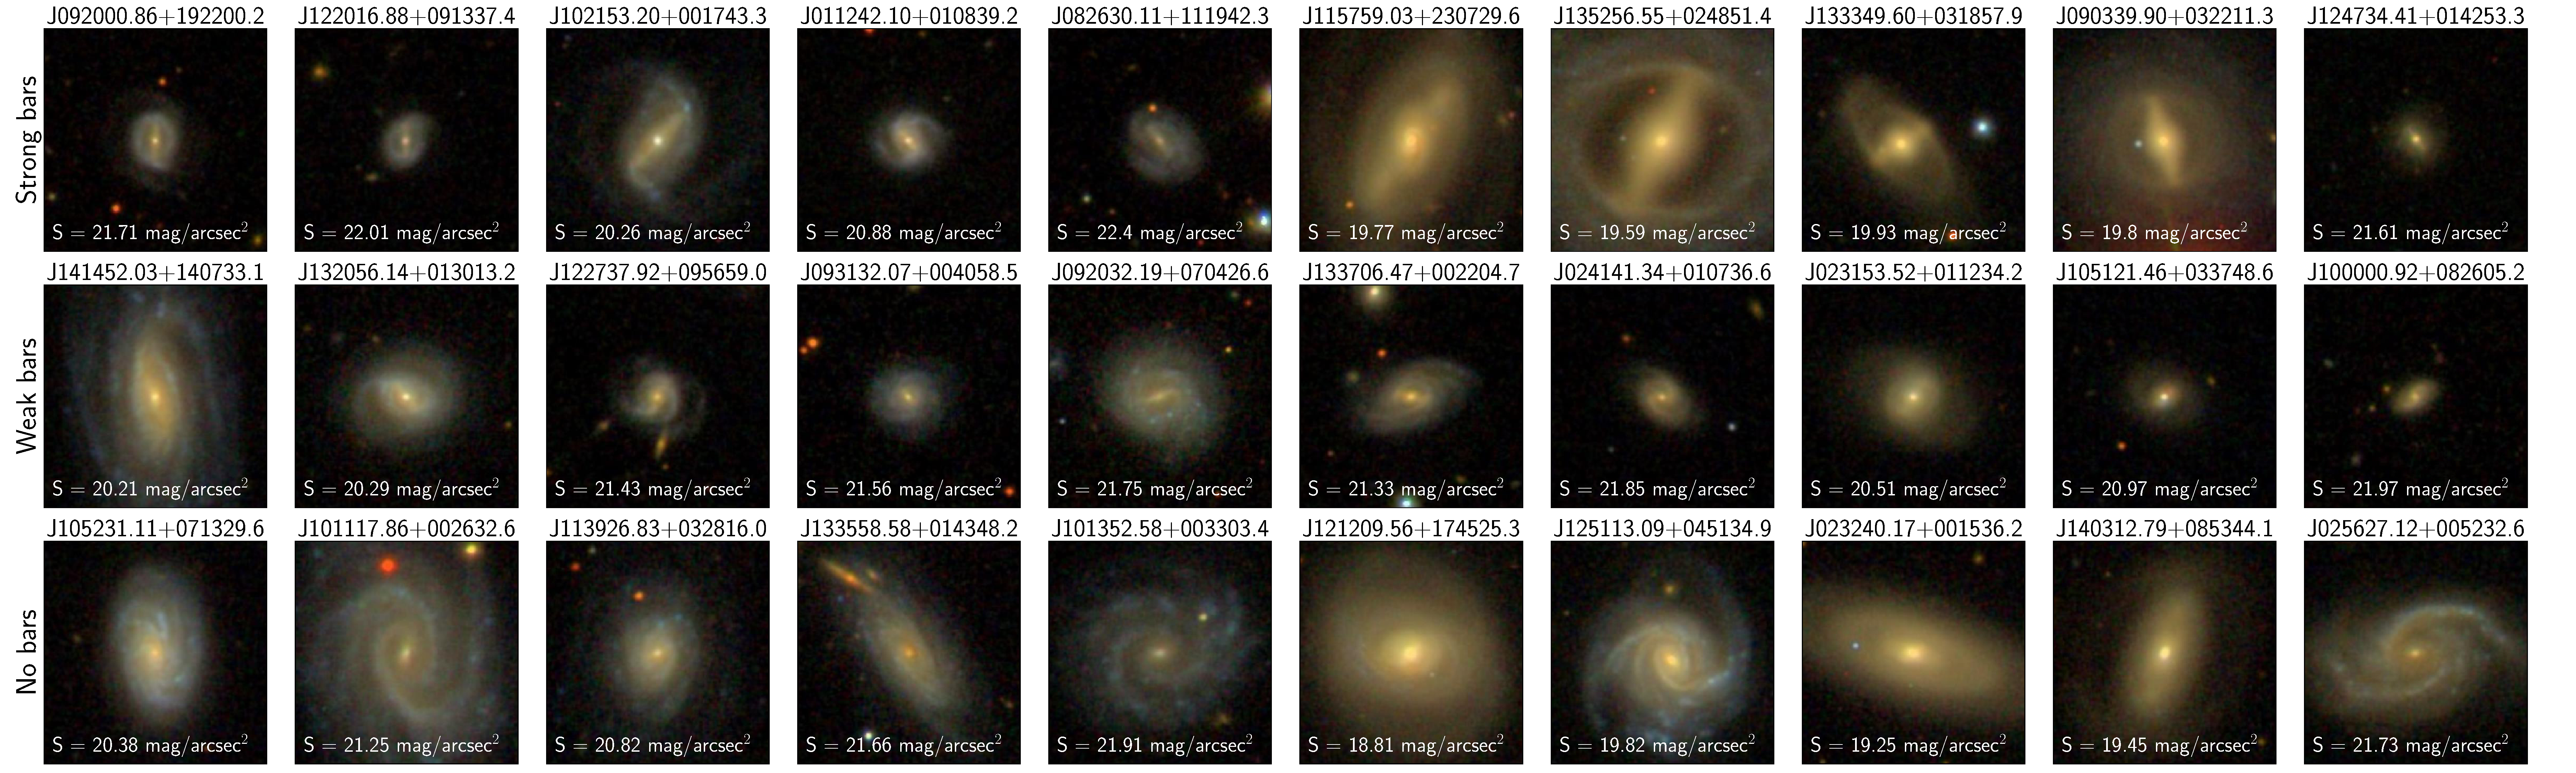
\includegraphics[width=0.8\textwidth]{fig_bars.pdf}}
\\
\begin{flushleft}
Figure 1: Mosaic of SDSS \emph{ugriz} postage stamps of targets in this sample ($0.01 < z < 0.05$). The sample is split into strong bars (top), weak bars (middle) and no bars (bottom; our control sample) which are mass-matched along each column. The surface brightness of each source is also noted. The 5 leftmost columns are galaxies in the blue cloud and the 5 rightmost columns are all galaxies in the red sequence (see Figure 2). Each image is 63 arcseconds across.
\end{flushleft}


% \centering{
% 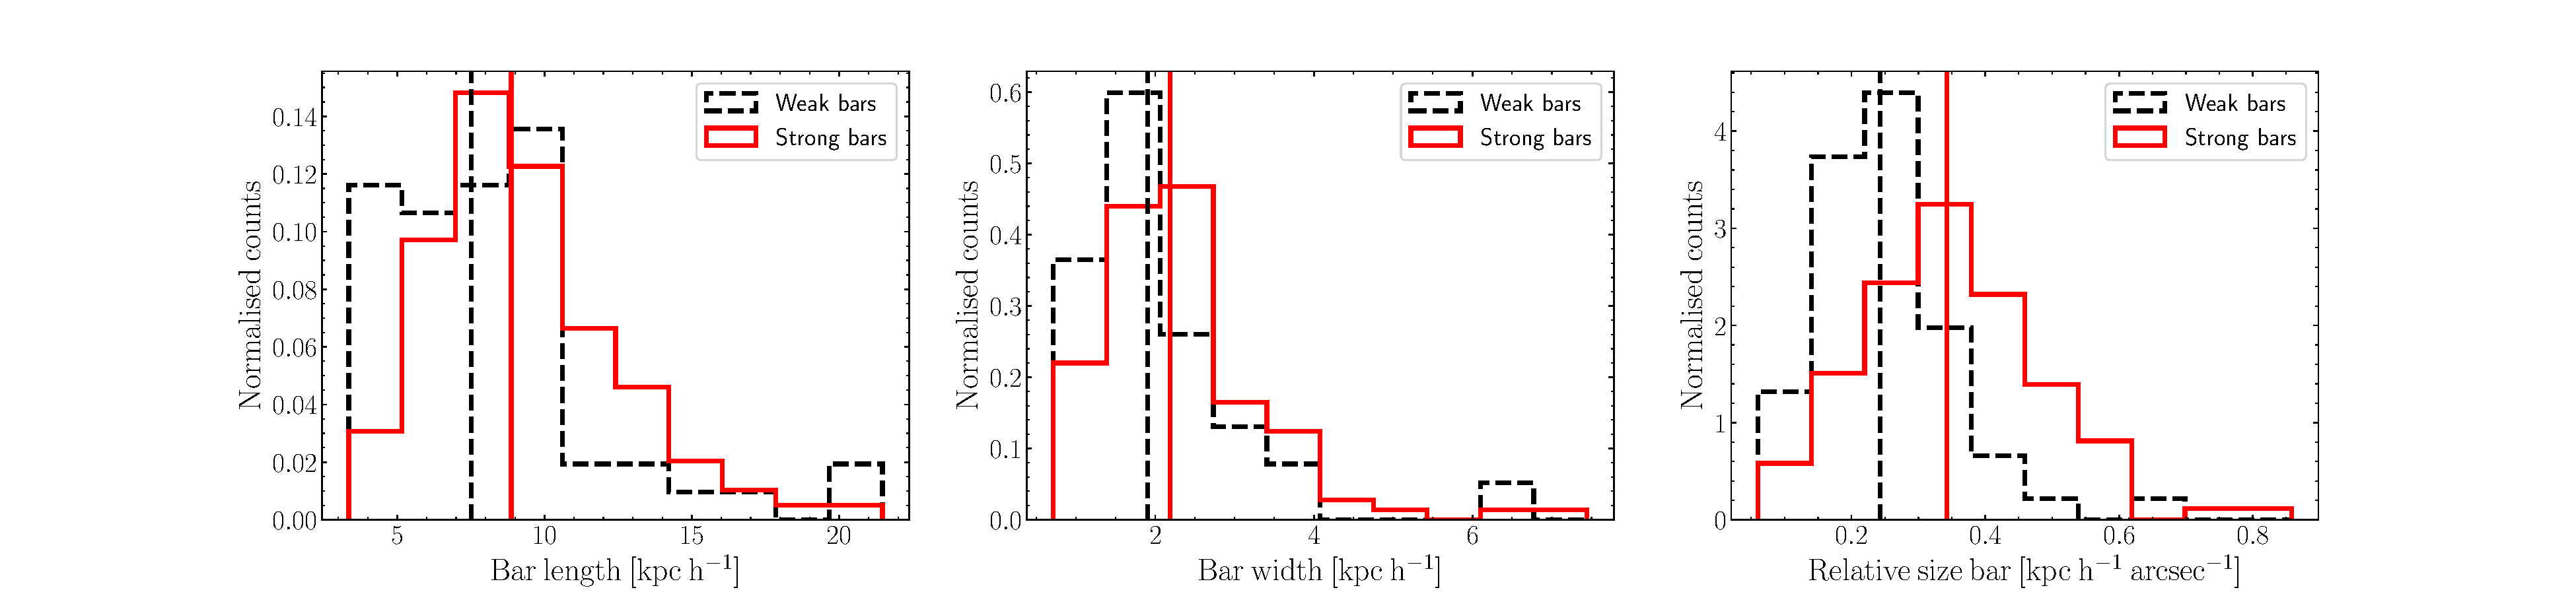
\includegraphics[width=0.6\textwidth]{obs_barlen.pdf}}
% %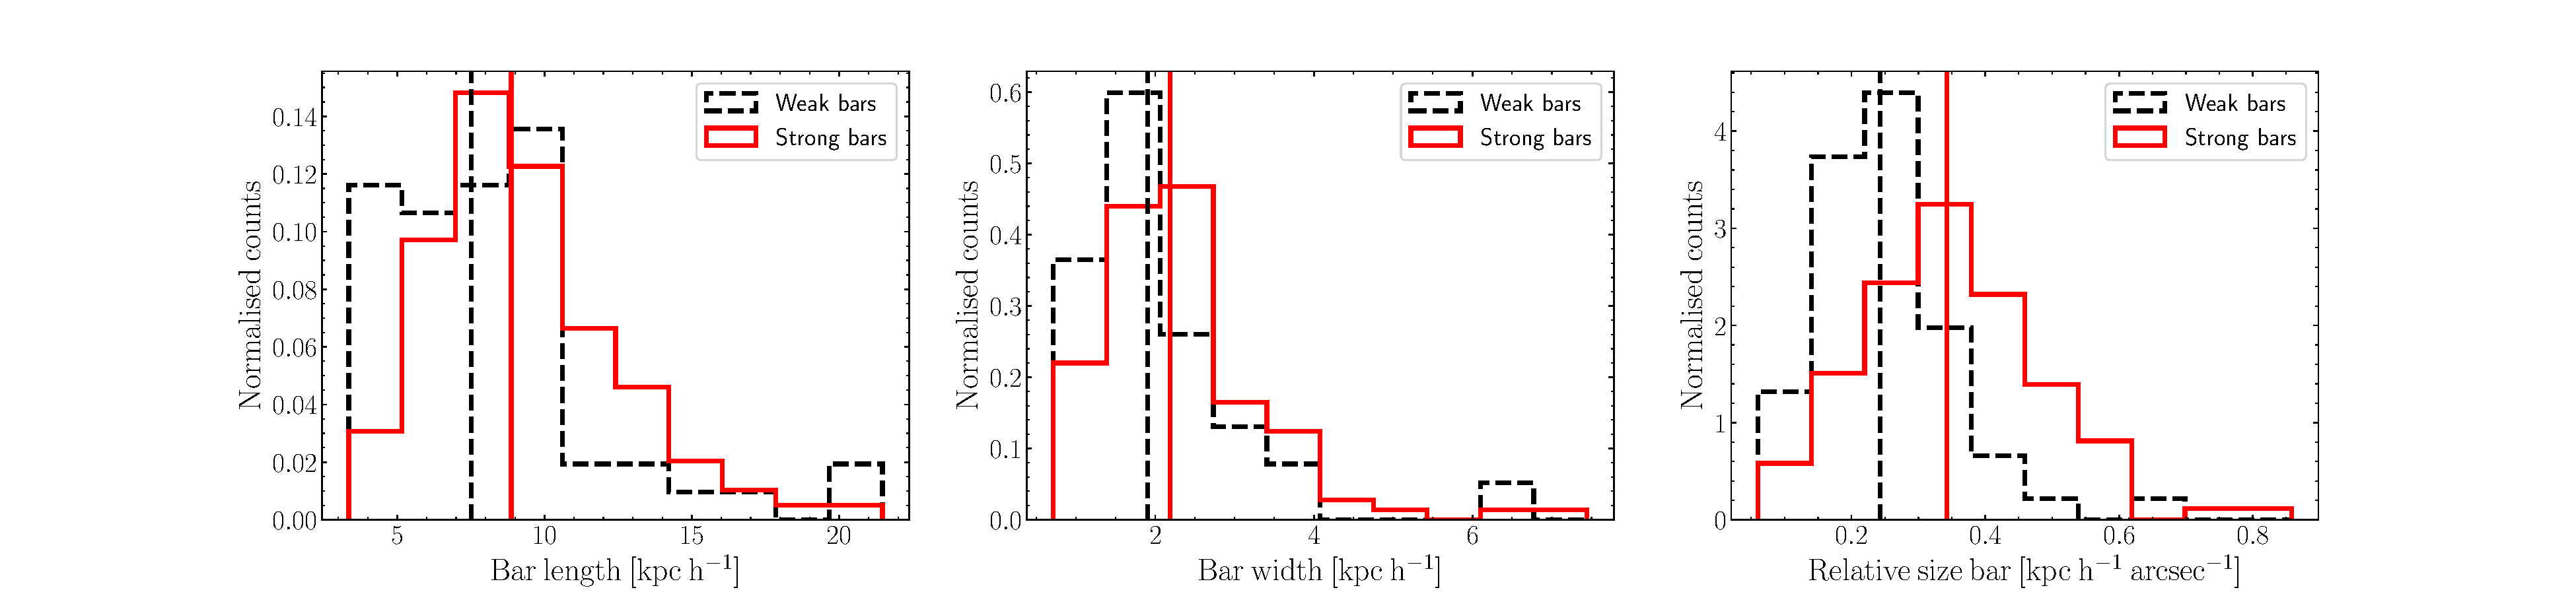
\psfig{file=obs_barlen.pdf ,width=17cm}\label{fig:histograms}
% \\
% \begin{flushleft}
% Figure 2: Distribution of the bar lengths (left; 2.4$\sigma$ difference), widths (middle; 1.8$\sigma$ difference) and relative size compared with the galaxy $r$-band Petrosian radius(right; 5.0$\sigma$ difference) for the parent sample from which our targets were selected which have bar size measurements (Hoyle et al. 2011$^{[3]}$). This figure shows that strong bars are distinct from weak bars, however this does not confirm whether they are distinct phenomenon. This proposal aims to test this hypothesis.
% \end{flushleft}
\begin{multicols}{2}
\centering {
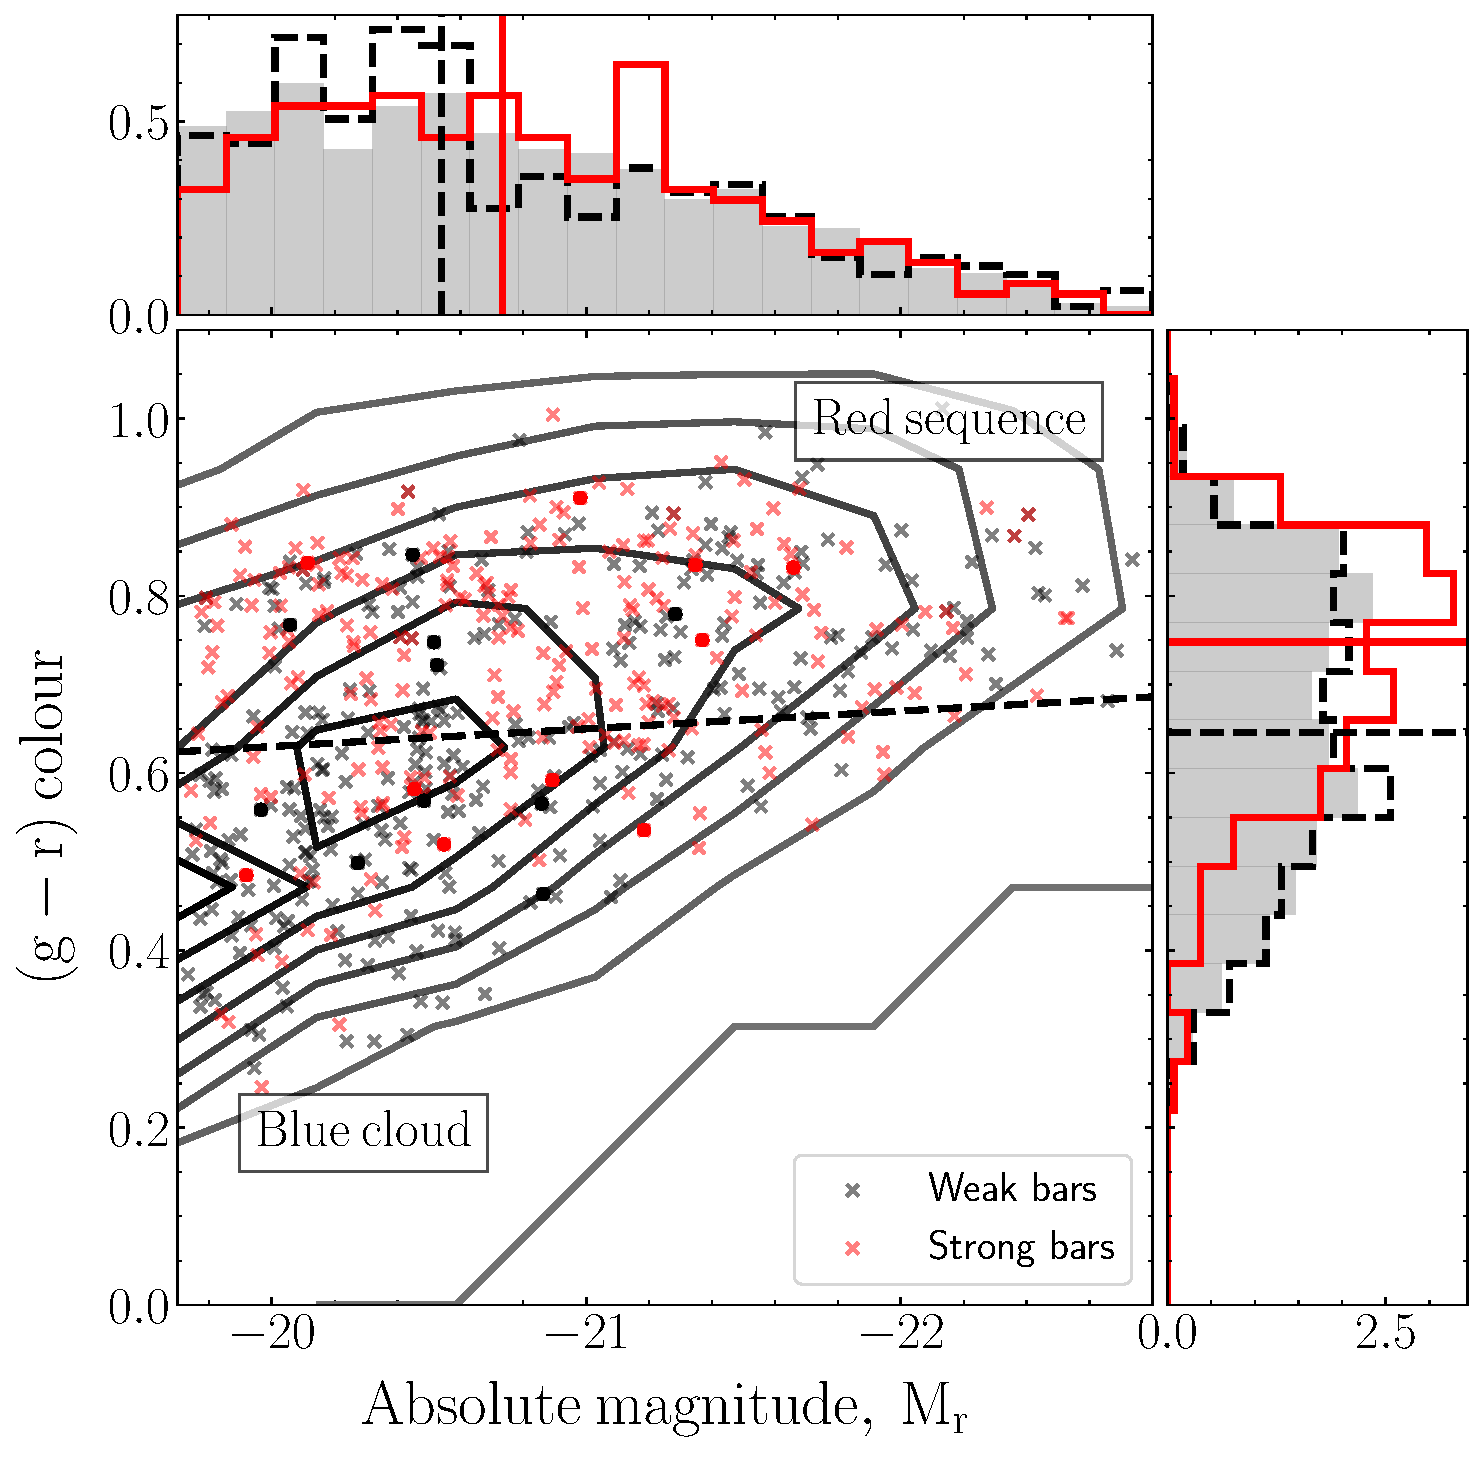
\includegraphics[width=0.45\textwidth]{obs_colmag.pdf}}
\\
\begin{flushleft}
Figure 2: Colour magnitude diagram showing the locations of strong (red crosses and histogram) and weak (black crosses and histogram) bars in the parent sample. Circles show targets in this proposal. We also show the overarching distribution of galaxies in SDSS across this plane (black contours and grey histogram). We see a significant difference between the distribution of colours in strong and weak bars; with strong bars found preferentially on the red sequence (68$\%$ of total strong bar population) and weak bars evenly distributed (6.7$\sigma$ and 0.27$\sigma$ difference from the overarching SDSS galaxy population for strong and weak bars, respectively). We therefore aim to test the hypothesis that strong bars cause the quenching of star formation, driving disc galaxies from the blue cloud to the red sequence, whereas weak bars do not. 
\end{flushleft}
\end{multicols}
%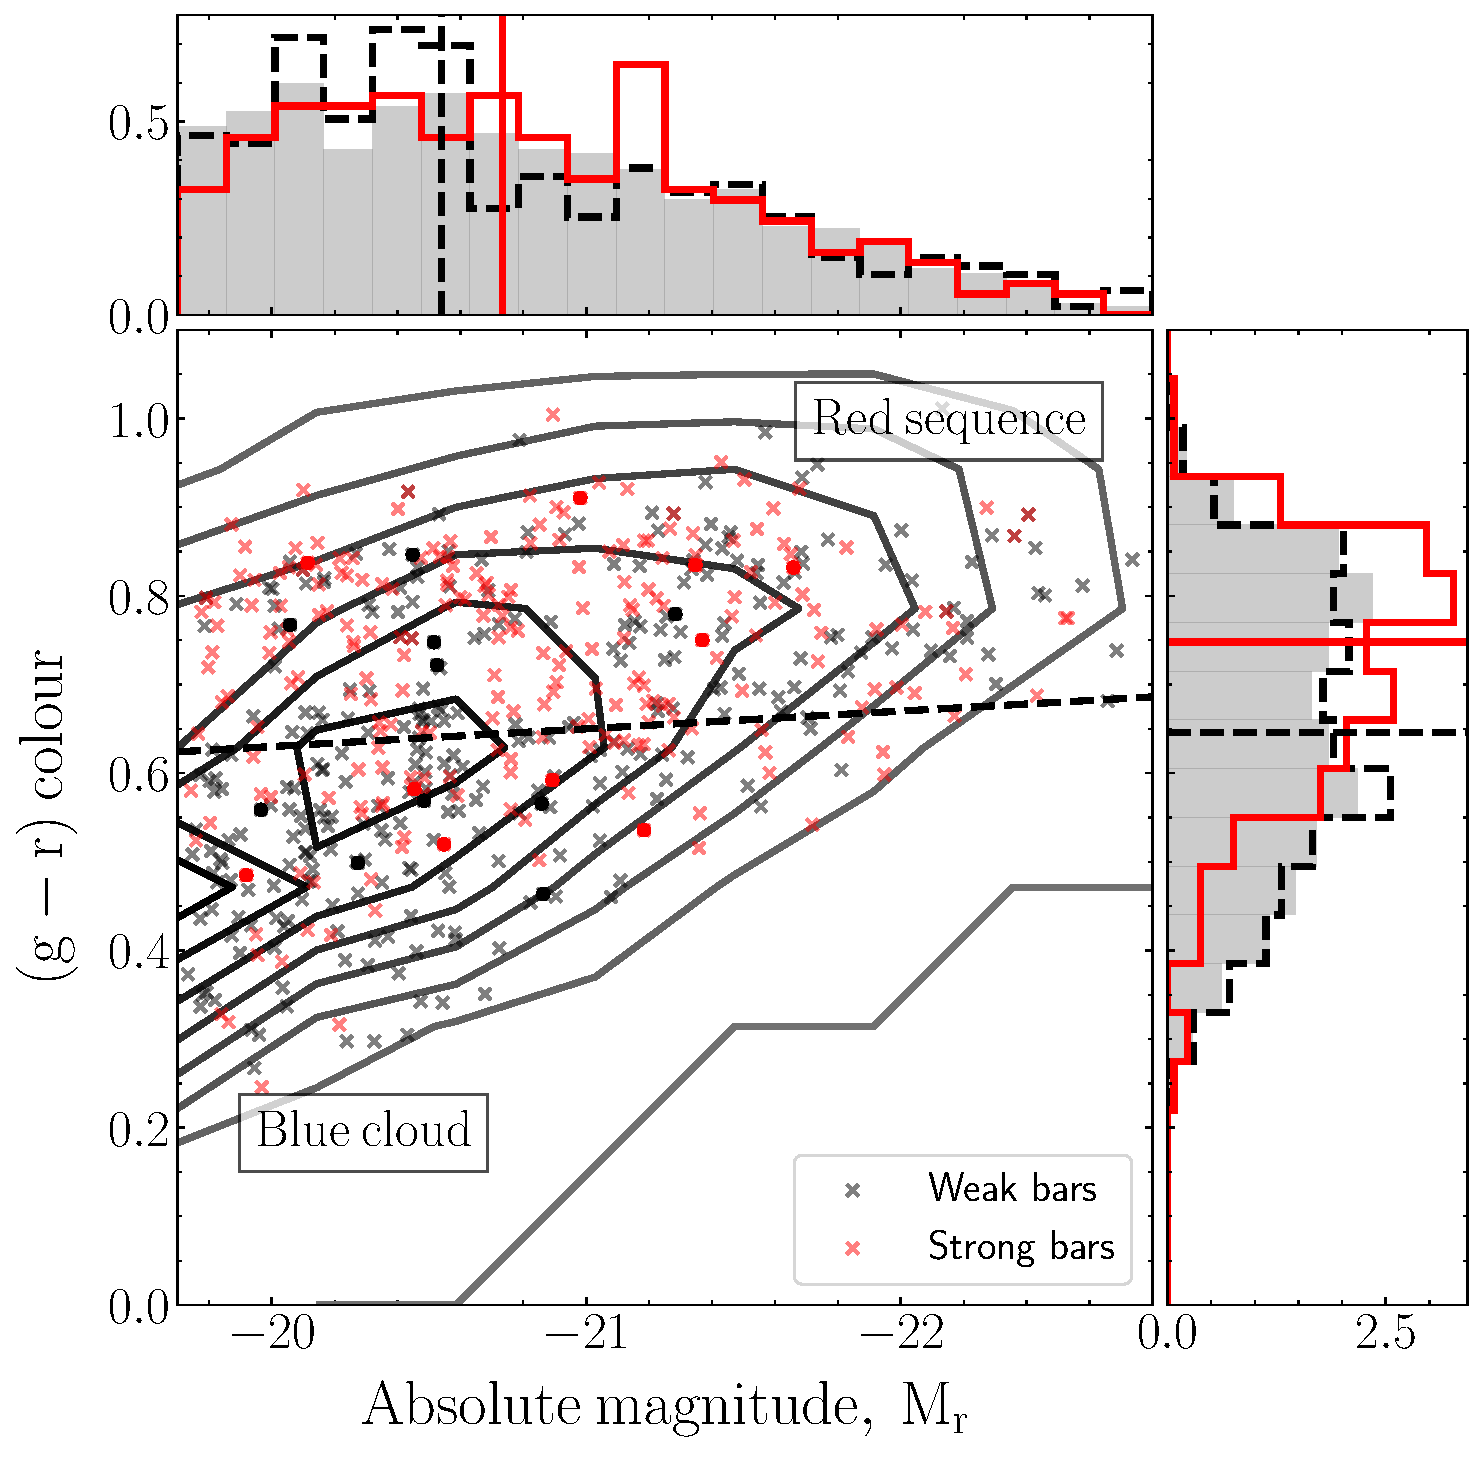
\psfig{file=obs_colmag.pdf,width=7.5cm}\label{fig:colmag}


% proposals written in a font smaller than 11pt will be rejected

}

%%%%%%%%%%%%%%%%%%%%%%%%
% PAGE 5 OF PATT2 FORM %
%%%%%%%%%%%%%%%%%%%%%%%%

\backupprogram{In the case of poor seeing we shall limit the number of sources targeted and increase exposure times in order to still achieve optimal signal-to-noise ratios for a selection of our targets (initally those with shorter calcualted exposure times). This will still allow the kinematics and star formation rates to be determined but in a reduced sample size.}             % Summary of backup programme

\previous{                   % Previous applications (last 4 Sems)
\begin{tabular}[t]{p{1.5in}p{0.7in}p{0.8in}p{3.2in}}
%Patt No. & Award & clear nights & comments \\
\end{tabular}
}

\publications     {}         % List pubs with data from patt time (last 4 Sems)

\experience       {}         % Experience of observers on other telescopes
\graduatestudent  {}{}       % Research student {Name of student}{Project}
\grant            {}{}{}     % {Name of PI}{Grant title}{Grant No.}
\nonstandardtravel{}         % Justify T&S for more than one UK observer
\otherexpenditure {}         % eg for freight etc.


%%%%%%%%%%%%%%%%%%%%%%%%%%%%%%%%%%%%%%%%%%%%%%%%%%%%%%%%%%%%%%%%%%%%%%%%%%%%%
% PAGE 6 OF PATT2 FORM - THIS SECTION IS REMOVED BY THE AAT DURING PROCESSING
% IF INCLUDED.  ING APPLICANTS SHOULD NOT ENTER ANYTHING HERE.
%%%%%%%%%%%%%%%%%%%%%%%%%%%%%%%%%%%%%%%%%%%%%%%%%%%%%%%%%%%%%%%%%%%%%%%%%%%%%

\shorttitle {}               % Ignore if you are an ING applicant.



\makepatttwopageone
\makepatttwopagetwo
\makepatttwopagethree

%%%%%%%%%%%%%%%%%%%%%%%%%%%%%%%%%%%%%%%%%%%%%%%%%%%%%%%%%%%%%%%%%%%%%
% COMMENT THE FOLLOWING LINE IN *ONLY* IF                           % 
%                                                                   %
% YOU ARE APPLYING FOR 8 OR MORE NIGHTS ON THE AAT, WHT OR UKIRT, OR% 
% YOUR PROPOSAL IS LONG-TERM FOR THE AAT, WHT, UKIRT OR INT, OR     % 
% YOUR PROPOSAL IS COORDINATED WITH OTHER TELESCOPES                % 
%                                                                   % 
% *AND* YOU HAVE USED THE CONTINUATION PAGE FOR YOUR SCIENTIFIC CASE% 
%%%%%%%%%%%%%%%%%%%%%%%%%%%%%%%%%%%%%%%%%%%%%%%%%%%%%%%%%%%%%%%%%%%%%
 
\makepatttwopagethreea

\makepatttwopagefour
\makepatttwopagefoura
\makepatttwopagefive

% FOR ING APPLICATIONS LEAVE THE FOLLOWING LINE COMMENTED OUT

%\makepatttwopagesix         

% FOR AAT APPLICATIONS YOU MAY LEAVE IT IN IF YOU WISH.  IT WILL NOT
% BE TRANSMITTED TO THE TAG HOWEVER.

\end{document}
